\documentclass{school-22.211-notes}
\date{May  2, 2012}

\begin{document}
\maketitle

\lecture{Nodal Diffusion Methods} \label{nodal-methods}
There has not been a single LWR core that was solved using discrete transport. As we will see later, the number of core hours needed to solve a LWR using discrete transport is approximately 100,000 core hours, whereas pin-by-pin diffusion with homogenized pin cells reduce the core hours by \uline{a factor of 100,000}.

\topic{3D Core Analysis Overview}
Reference: \href{www.oecd-nea.org/dbprog/documents/MC03Smith.pdf}{`Reactor Core Methods' by Smith, MC 2003}.

\subtopic{Challenges} 
There are a couple levels of complexity for performing 3D core analysis,
\begin{itemize}
\item One reactor at one state point: couple core neutronics/fuel heat conduction/coolant hydraulics/structural mechanics for 60,000 fuel pins and 100 axial levels to evaluate thermal margins;
\item Repeat for 50 depletion states and track 300 isotopes;
\item Repeat for 10,000s limiting conditional simulations and 100s of transient accident simulations for safety analysis;
\item Repeat for 1000s of startup and maneuver simulations;
\item Repeat for millions of cycle depletion simulation for designing loading design and optimization;
\item For operator training simulator in real time, 24/7 operation at 5-10 Hz. 
\end{itemize}
The challenges for 3D core calculation include,
\begin{itemize}
\item Predict pin power, axial shapes of pin power: as in Figure~\ref{3Dcore}, the spacers depress the flux. Though even without the spacers, the axial shape would still be more towards the bottom compare with a cosine shape due to the temperature coefficients; 
\item Predict core reactivity with core burnup: as in Figure~\ref{3Dcore}, burnable poisons deplete as burnup increases;
\item Predict in-core detector response;
\item Predict control rod worths and temperature coefficients. 
\end{itemize}
\begin{figure}[ht]
  \centering
  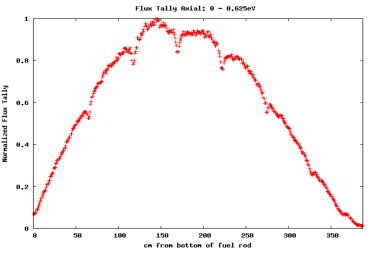
\includegraphics[width=3in]{images/methd/3Dcore-spacer.png}
  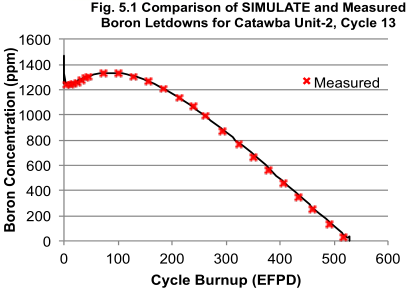
\includegraphics[width=3in]{images/methd/3Dcore-poison.png}
  \caption{3D Core Calculation Samples} \label{3Dcore}
\end{figure}

\subtopic{Approaches to 3D core Problems}
\begin{enumerate}
\item  Discrete Transport: the number of meshes we need is approximately
\eqn{ 100 \frac{\mathrm{mesh}}{\mathrm{pin}} \times 300 \frac{\mathrm{pins}}{\mathrm{assembly}} \times 200 \frac{\mathrm{assemblies}}{\mathrm{core}}\times 100 \mbox{ axial mesh}\times 100 \mbox{ energy groups}\times 1000 \mbox{ angles} = 6 \times 10^{13} }
The best parallel transport grind time currently comes from Texas A\&M PDT code is 300 nanosecond/unknown. On top of that, assume we perform 20 fission source iterations, we are looking at \uline{100,000 core hours}. Not to mension that we have no inlcude thermal-hydraulic feedback, cross section evaluations, boron search to criticality, equilibrium xenon, and control rod search to criticality. 

\item Pin-by-pin diffusion with homogenized pin cells: the number of meshes we need is approximately 
\eqn{ 1 \frac{\mathrm{mesh}}{\mathrm{pin}}\times 300 \frac{\mathrm{pins}}{\mathrm{assembly}}\times 200 \frac{\mathrm{assemblies}}{\mathrm{core}}\times 100 \mbox{ axial mesh} 100 \times\mbox{ energy groups}\times 1 \mbox{ angles} = 6 \times 10^{8} }
Thus we reduce the core hours from 100,000 to 1 core hour. The drawback is that pin homogenization causes a loss of accuracy around strong absorbers. This is now a tractable problem, but not used for production.

\item Nodal method: this is what production codes typically use. There is a huge push towards nodal method, because nodal methods take a mesh size of 20cm to be accurate, whereas Finite Difference method requires a mesh size of about 1 cm. In terms of the amount of errors, using CMFD on a reactor application would yield somewhere between 5-10\% error. 
\end{enumerate}

\textbf{Multilevel Approach} for LWRs (the reason we emphasize this approach is for LWRs is because the spatial mesh should agree with mean free path which depends on energies):
\begin{enumerate}
\item Spectral code to get from 1000s of energy groups to 100s of energy groups. 
  \begin{enumerate}
    \item Pin cell or homogenized medium. 
    \item 0D or 1D spatial model.
  \end{enumerate}

\item Solve each unique lattice. 
  \begin{enumerate}
  \item Self-shielding corrections. 
  \item 2D transport theory (100s energy groups). 
  \item Homogenize parameters.
  \end{enumerate}

\item Solve nodal diffusion (3D diffusion equation with few energy groups). 
\end{enumerate}
For fast reactors, we solve a lattice with 10,000 groups and go straight to diffusion (with 30-40 energy groups) because the mean free path is so long. 


\clearpage
\subtopic{PWR Methods: A Historical Review}
\begin{enumerate}
\item Early 60s, core analysis were done using 2D/1D finite diffusion calculation. For steady state,
  \begin{enumerate}
  \item Pin-cell cross section generation (e.g.: Westinghouse's Leopard), uses supercell for absorbers (absorber/fuel buffer pin-cell). 
  \item Radial shape generatoin (e.g., PDQ/HARMONY): generate 2-group homogenized pin cell F-xy peaking (axial plane peaking) using finite difference diffusion with no feedback 
  \item Axial: generate A-O (axial offset) and $F(z)$ axial shape using 2 group 1D axial finite difference diffusion. 
  \end{enumerate}
  Transient analysis: 0D point kinetics with feedback, 1D axial 2 group, finite difference diffusion with feedback, then we superimpose the steady state radial peaking to get the 3D peaking: $F(z) \times$ F-xy. 

\item Mid-60s: users want direct 3D computations, thus we do 3D steady-state multigroup neutron diffusion equation. 
  \begin{enumerate}
  \item Mesh spacing: needs $< 1\cm$ to be accurate. 
  \item FLARE BWR Nodal model (1964): one energy group, a source in node $p$ is related to itself and its six neighboring node $q$: 
    \eqn{ S^p = \frac{\kinf^p}{\lambda} (w_{pp} S^p + \Sum_{q=1}^6 w_{qp} S^q ) }
    where the migration coefficients $M_p^2 = \frac{D_p}{\Sigma_p}$, $g$ is an adjustable parameter, and the coupling coefficients are $\displaystyle w_{pq} = (1-g) \frac{\sqrt{M_p^2}}{2h} + g \frac{M_p^2}{h^2}, w_pp = 1 - \Sum_{q=1^6} w_{pq}$. 
    There is not much physics in this model, because the coefficients are derived assuming two infinite half planes. 
  \end{enumerate}

  \item 70s-80s advanced nodal diffusion methods. 
    \begin{enumerate}
    \item Goals: 
      \begin{itemize}
      \item Directly represent baffle/reflector, instead of like previous codes that just use screw-driver to account for the albedos; 
      \item No user-adjusted parameters, should be all physics; 
      \item Full 3D thermal-hydraulic feedback by assemblies;
      \item Recover individual pin powers; 
      \end{itemize}

    \item In Germany: KWU became Siemens who became Areva, and they have two version of the nodal diffusion method: 
      \begin{itemize}
        \item NEM: Wagner, Koebke, Winter et. al. 
        \item CUBOX/QUABOX: Finnemann. 
      \end{itemize}

    \item At MIT:     
      \begin{itemize}
      \item Prof. Kent Hansen was working on FEM (finite element method), which turned out to be limited because the methods are more complex compared with nodal methods. 
      \item Prof. Allan Henry's group did ANM-1D analytic, NEM variants, ANM-FLT, and QUANDRY. 
      \end{itemize}

    \item At University of Illinois, Prof. Jack Dorning's group has NGFM. 
    \end{enumerate}

  \item Modern advance nodal codes: there are numerous of them, and they should all be the same. Specific code names are listed in Lec 19 in 22.212. 
\end{enumerate}


\clearpage
\topic{Derivation of Nodal Balance Equation}
Reference: Sutton and Aviles' `Diffusion Theory Methods for Spatial Kinetics Calculations' (1996). 

To start, \hi{nodal methods are just a way of providing the higher-order coefficients that describe the net current in terms of node-averaged fluxes}: 
\eqn{ J = - \frac{2D^+ D^-}{D^- h^+ + D^+ h^-} (\phi^+ - \phi^-) }
where nodal methods is no better than the $\frac{2D^+ D^-}{D^- h^+ + D^+ h^-}$. 

Next we derive the nodal balance equations. 
\begin{enumerate}
\item We start from 3D steady-state multigroup neutron diffusion equation, 
  \eqn{\divergence \vecJ_g(\vecr, E) + \Sigma_{rg} \psi_g (\vecr, E) = \frac{1}{\keff} \chi_g \Sum_{g' = 1}^G \nu \Sigma_{fg'} \psi_{g'}(\vecr, E) + \Sum_{g'=1}^G \Sigma_{sg'g} \psi_{g'}(\vecr, E) }
  Apply Fick's Law of diffusion for current out of flux, 
  \eqn{ \vecJ_g(\vecr, E) = - D_g(\vecr, E) \gradient \psi_g(\vecr, E) }

\item Volume average of diffusion equation for a node: we integrate every term over the node volume then divide by volume. The volume averaged flux becomes, 
  \eqn{ \bar{\psi} = \frac{1}{h_x h_y h_z} \int_0^{h_x} \int_0^{h_y} \int_0^{h_z} \psi(x,y,z) \dx \dy \dz }

\item The leakage term becomes (after integrating the divergence term using Gauss Theorem), 
  \eqn{ \int_0^{h_x} \int_0^{h_y} \int_0^{h_z} \divergence \vecJ_g \dx \dy \dz &= \int_0^{h_y} \int_0^{h_z} (J_x(h_x,y,z) - J_x(0,y,z)) \dy \dz  \\
&+ \int_0^{h_x} \int_0^{h_z} (J_y (x,h_y, z) - J_y(x,0,z)) \dx \dz \\
&+ \int_0^{h_x} \int_0^{h_y} (J_z(x,y,h_z) - J_z(x,y,0)) \dx \dy }
  If we define surface-averaged currents, 
  \eqn{ \bar{J}_{gxl} &= \frac{1}{h_y h_z} \int_0^{h_y} \int_0^{h_z} J_x(0,y,z) \dy \dz, & \bar{J}_{gxr} &= \frac{1}{h_y h_z} \int_0^{h_y} \int_0^{h_z} J_x(h_x,y,z) \dy \dz }
  Then the leakage term becomes, 
  \eqn{ \Sum_{u=x,y,z} \frac{\bar{J}_{gur} - \bar{J}_{gul}}{h_u} }
 
\item Together, the nodal balance equation with average terms is, 
  \eqn{ \Sum_{u=x,y,z} \frac{\bar{J}_{gur} - \bar{J}_{gul}}{h_u} + \Sigma_{rg} \bar{\psi}_g &= \frac{1}{\keff} \chi_g \Sum_{g'=1}^G \nu \Sigma_{fg'} \bar{\psi}_{g'} + \Sum_{g'=1}^G \Sigma_{sg'g} \bar{\psi}_{g'} \label{nodal-balance} }
  Notice, 
  \begin{itemize}
    \item Formally, we have not approximate yet. 
    \item The six surface-averaged currents are required to find the node-averaged flux which would determine nodal power;
    \item Surface-averaged currents are average of flux derivative on a surface, which equals derivative of average flux at the surface; 
    \item It is more efficient to work with diffusion equation for average flux rather than solving the diffusion equation for the point-wise fluxes in 3D. 
  \end{itemize}
\end{enumerate}


\clearpage
\topic{Representing Interface Current in 1D}
As we mentioned above, the nodal balance equation we arrived at Eq.~\ref{nodal-balance} is exact thus far. The next step is to represent the net current in terms of node-averaged fluxes. In 1D, for instance, we use two-node two-group finite difference scheme as an example: 
\begin{figure}[h]
  \hspace{-1in}
  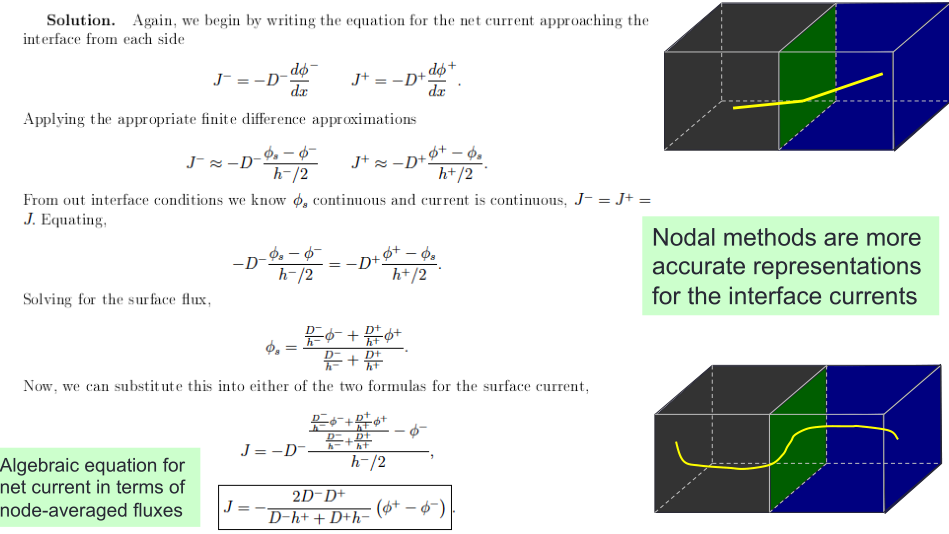
\includegraphics[width=1.2\textwidth]{images/methd/2node2g-finite-difference.png}
\end{figure}



\clearpage
\topic{Representing Interface Current in 3D: Transverse Integration}
We need a set of equations for the surface average currents instead of solving 3D finite different equations directly. The general idea is, 
\begin{itemize}
\item In approaching surface averaged current, the average of flux derivative on a surface is approximated as the derivative of average flux at the surface. 

\item It is more efficient to work with the diffusion equation for average flux rather than diffusion equation for 3D point wise fluxes. 

\item We use the transverse integration scheme to approach the 3D diffusion equation: We pick a direction of interest (eg., x direction), and perform integration within node over 2D plane normal to that direction (eg., the grey surface in Figure~\ref{nodal-current}), then devide by the planar area. 
\begin{figure}[ht]
  \centering
  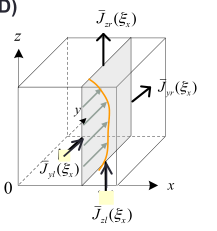
\includegraphics[width=0.28\textwidth]{images/methd/nodal-current.png}
  \caption{Integrate Within Node Over 2D Plane Normal to x-direction} \label{nodal-current}
\end{figure}
\end{itemize}

Next we discuss the details of transverse integration of the 3D diffusion equation. 
\begin{enumerate}
\item The LHS of Eq.~\ref{nodal-balance} becomes, 
  \eqn{ \mathrm{LHS} = \frac{1}{h_y h_z} \int_0^{h_z} \int_0^{h_y} \lp \divergence \vec{J}_g(\vecr, E) + \Sigma_{rg} \bar{\psi}_g \rp \dydz }

\item The RHS becomes not interesting after a while because it is just the average flux times cross sections. 

\item Define dimensionless independent variables,
  \eqn{ \xi_x &= \frac{x}{h_x}, & \xi_y &= \frac{y}{h_y}, & \xi_z &= \frac{z}{h_z} }
  and we can transform the integration and the derivative operator as well, 
  \eqn{ \frac{\du}{h_u} &= \derivative \xi_u, & \ddu &= \frac{1}{h_u}\frac{\derivative}{\dxi_u}, & u&= x,y,z}

\item Simplify the averaging with dimensionless variables ($l$ is left, $r$ is right): we basically say the net current on the left plane can be found by integrating the 3D net current at $x=0$ over the left plane. 
  \eqn{ J_{xgl} &= \int_0^1 \int_0^1 J_x(0,\xi_y, \xi_z) \dxi_y \dxi_z, &J_{gxr} &= \int_0^1 \int_0^1 J_x(1,\xi_y, \xi_z) \dxi_y \dxi_z }
  \eqn{ \bar{\psi} &= \int_0^1 \int_0^1 \int_0^1 \psi(\xi_x, \xi_y, \xi_z) \dxi_x \dxi_y \dxi_z }

\item We recall the normalized 3D diffusion equation, 
  \eqn{ \left( - \Sum_{u=x,y,z} \frac{D_g}{h_u^2} \frac{\partial^2}{\partial \xi_u^2} + \Sigma_{rg} \right) \psi_g(\xi_x, \xi_y, \xi_z) &=  \frac{1}{\keff} \chi_g \Sum_{g'=1}^G \nu \Sigma_{fg'}\psi_g(\xi_x, \xi_y, \xi_z) + \Sum_{g'=1}^G \Sigma_{sg'g} \psi_g(\xi_x, \xi_y, \xi_z) }

\item We look at the leakage term after the transverse integration, notice that at the end of the day terms only depend on $x$ direction becuse we integrate away the corerwponding $y$ and $z$ directions:
  \begin{align}
    &\int_0^1 \int_0^1 \divergence \vecJ \dxi_y \dxi_z = \int_0^1 \int_0^1 \left( \frac{1}{h_x} \frac{\partial J_x}{\partial \xi_x} + \frac{1}{h_y} \frac{\partial J_y}{\dxi_y} + \frac{1}{h_z} \frac{\partial J_z}{\dxi_z} \right) \dxi_y \dxi_z \\
    &= \int_0^1 \int_0^1 \left( -\frac{D_g}{h_x^2} \frac{\partial^2 \psi}{\partial \xi_x^2} + \frac{1}{h_y} \frac{\partial J_y}{\dxi_y} + \frac{1}{h_z} \frac{\partial J_z}{\dxi_z} \right) \dxi_y \dxi_z \\
    &= - \frac{D_g}{h_x^2} \frac{\partial^2 }{\partial \xi_x^2} \int_0^1 \int_0^1 \psi(\xi_x, \xi_y, \xi_z) \dxi_y \dxi_z \\
    &+ \frac{1}{h_y} \int_0^1 (J_y(\xi_x, 1, \xi_z) - J_y(\xi_x, 0, \xi_z) )\dxi_z + \frac{1}{h_z} \int_0^1 (J_z(\xi_x, \xi_y, 1) - J_z(\xi_x, \xi_y, 0) ) \dxi_y \\
    &= - \frac{D_g}{h_x^2} \frac{\partial \bar{\psi}_x (\xi_x)}{\partial \xi_x^2} + \frac{\bar{J}_{yr}(\xi_x) - \bar{J}_{yl} (\xi_x)}{h_y} + \frac{\bar{J}_{zr} (\xi_x) - \bar{J}_{zl} (\xi_x)}{h_z} 
  \end{align}
  where we defined the \textbf{plane-averaged 1D flux}, and it does not have mesh spacing on the bottom because we defined dimentionless terms:
  \eqn{\bar{\psi}_x = \int_0^1 \int_0^1 \psi(\xi_x, \xi_y, \xi_z) \dxi_y \dxi_z }
  and \textbf{line-averaged surface current} at an arbitrary position $\xi_x$, 
  \eqn{ \bar{J}_{yr} (\xi_x) &= \int_0^1 J_y(\xi_x, 1, \xi_z) \dxi_z, &\bar{J}_{yl}(\xi_x) &= \int_0^1 J_y(\xi_x, 0, \xi_z) \dxi_z }
  \eqn{ \bar{J}_{zr} (\xi_x) &= \int_0^1 J_z(\xi_x, \xi_y, 1) \dxi_y, &\bar{J}_{zl}(\xi_x) &= \int_0^1 J_z(\xi_x, \xi_y,  0) \dxi_y }

\item Collect all the terms, we get the transverse integration of 3D diffusion equation, 
  \eqn{ \Sum_{u=y,z} \frac{\bar{J}_{gur}(\xi_x) - \bar{J}_{gul}(\xi_x)}{h_u} - \frac{D}{h_x^2} \frac{\derivative^2}{\dxi_x^2} \bar{\psi}_{gx} (\xi_x) + \Sigma_{rg} \bar{\psi}_{gx} (\xi_x) &=  \frac{1}{\keff} \chi_g \Sum_{g'=1}^G \nu \Sigma_{fg'}\psi_g(\xi_x) + \Sum_{g'=1}^G \Sigma_{sg'g} \psi_g(\xi_x)  }
  If we define a \textbf{transverse leakage term} (the source that comes in the plane) and move it to the RHS, 
  \eqn{ L_{gu}(\xi_x) &= \frac{1}{h_u} \left( \bar{J}_{gur}(\xi_x) - \bar{J}_{gul}(\xi_x) \right), & u &= y,z }
  and also define the \textbf{diffusion equivalent group constant}, 
  \eqn{ \Sigma_{Dg}^x  = \frac{D}{h_x^2} }
  We get the transverse integrated 1D diffusion equation, with two additional terms that describe the leakage in the other two directions. If we know the two leakage terms exactly, then we can solve the 1D diffusion equation exactly. 
  \eqn{ \boxed{ - \Sigma_{Dg}^x \frac{\derivative^2}{\dxi_x^2} \bar{\psi}_{gx} (\xi_x) + \Sigma_{rg} \bar{\psi}_{gx} (\xi_x) = \frac{1}{\keff} \chi_g \Sum_{g'=1}^G \nu \Sigma_{fg'} \bar{\psi}_{g'x} (\xi_x) + \Sum_{g'=1}^G \Sigma_{sg'g} \bar{\psi}_{g'x} (\xi_x) - L_{gy} (\xi_x) - L_{gz} (\xi_x)  }  }

\item Repeat for the other two directions, we get a set of 3 directional 1D diffusion equations.
  \begin{align}
    \boxed{ - \Sigma_{Dg}^x \frac{\derivative^2}{\dxi_x^2} \bar{\psi}_{gx} (\xi_x) + \Sigma_{rg} \bar{\psi}_{gx} (\xi_x) = \frac{1}{\keff} \chi_g \Sum_{g'=1}^G \nu \Sigma_{fg'} \bar{\psi}_{g'x} (\xi_x) + \Sum_{g'=1}^G \Sigma_{sg'g} \bar{\psi}_{g'x} (\xi_x) - L_{gy} (\xi_x) - L_{gz} (\xi_x) } \notag \\
    \boxed{ - \Sigma_{Dg}^y \frac{\derivative^2}{\dxi_y^2} \bar{\psi}_{gy} (\xi_y) + \Sigma_{rg} \bar{\psi}_{gy} (\xi_y) = \frac{1}{\keff} \chi_g \Sum_{g'=1}^G \nu \Sigma_{fg'} \bar{\psi}_{g'y} (\xi_y) + \Sum_{g'=1}^G \Sigma_{sg'g} \bar{\psi}_{g'y} (\xi_y) - L_{gz} (\xi_y) - L_{gx} (\xi_y) }  \notag \\
    \boxed{ - \Sigma_{Dg}^z \frac{\derivative^2}{\dxi_z^2} \bar{\psi}_{gz} (\xi_z) + \Sigma_{rg} \bar{\psi}_{gz} (\xi_z) = \frac{1}{\keff} \chi_g \Sum_{g'=1}^G \nu \Sigma_{fg'} \bar{\psi}_{g'z} (\xi_z) + \Sum_{g'=1}^G \Sigma_{sg'g} \bar{\psi}_{g'z} (\xi_z) - L_{gx} (\xi_z) - L_{gy} (\xi_z) } \notag
  \end{align}

\item Interpretations: 
  \begin{itemize}
  \item We turn a 3D partial differential equation into three 1D ordinary differential equation that are coupled through average transverse leakage term. 
  \item It is exact if the transverse leakage shape is known. 
  \item Why nodal methods work? As the node becomes bigger and bigger, it is less likely that a random neutron to stream right through the node (thus contributing to the $\vecJ$). That is, \hi{$\vecJ$ streaming out the node from the right side is insensitive to the transverse leakage term from the top and the bottom.} Thus we can decouple leakage into three dimensions at large meshes. 
  \end{itemize}

\item \textbf{Approximation On Transverse Leakage: Quadratic Approximation in Each Node} (Finnemann, KWU). 
 From observation, flux is insensitive to the transverse leakage shape, so we are going to perform a quandrature polynomial with 2nd order polynomials of the leakage term, and iteratively update them. Quadratic approximation in each node, 
  \eqn{ L(\xi) = \bar{L} + l_1 P_1(\xi) + l_2 P_2(\xi) }
  \begin{figure}[h]
    \centering
    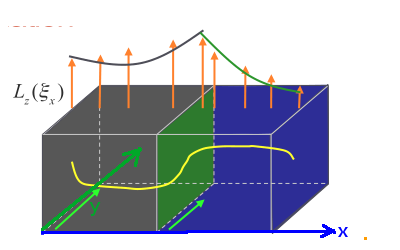
\includegraphics[width=4in]{images/methd/tl-approx.png}
    \caption{Transverse Leakage Approximation} 
  \end{figure}
  We apply average TL conservation scheme to determine $l_1, l_2$. We use three node average transver leakages (the values of each node and its two adjacent nodes), and impose constraint of conserving the averages of two adjacent nodes as in Fig.~\ref{tl-constrains}. Notice the parabola defined by the quadratic polynomial is assumed to extend over three nodes, but is only used in the middle node to represent the transverse leakage shape. Alternative approach: Finnemann (1977) uses continuity on transver leakage and its first derivative to determine the quadratic coefficients. 
    \begin{figure}[h]
    \centering
    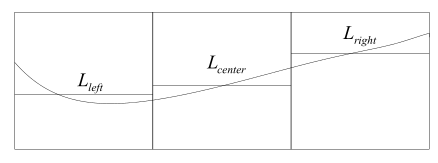
\includegraphics[width=4in]{images/methd/tl-constrains.png}
    \caption{Constraints on Transverse Leakage} \label{tl-constrains}
  \end{figure}
\end{enumerate}
About how we handle the rest of this method, we present three methods in the following sections. 


%%%%%%%%%%%%%%%%%%%%%%%%%%
\clearpage
\topic{Nodal Expansion Method (NEM)}
NEM was developed by Finnemann (KWU 1975). 
  \begin{enumerate}
  \item We approximate 1D flux by 4th order polynomial, 
    \eqn{ \bar{\psi}(\xi) = \Sum_{i=0}^4 a_i P_i (\xi) }
    where the basis functions are, 
    \begin{align}
      P_0(\xi) &= 1 \\
      P_1(\xi) &= 2 \xi - 1\\
      P_2(\xi) &= 6 \xi (1-\xi) - 1 \\
      P_3(\xi) &= 6 \xi (1-\xi)(2\xi-1) \\
      P_4(\xi) &= 6 \xi (1-\xi)(5\xi^2 -5\xi +1)
    \end{align}
    Notice these basis functions are not orthogonal, and integration from 0 to 1 would result in zero which is why we choose these basis (we should use these basis for 22.212 HW9). Keep in mind that our transverse leakage is 2nd order (because the result is not very sensitive to the expansion of the transverse leakage). 

  \item BCs: In a two nodes case, we have 16 unknowns from: 4 flux moments $\times$ 2 nodes $\times$ 2 energy groups. But we only have 8 knowns, 
    \begin{itemize}
      \item 4 node average fluxes: 2 groups $\times$ 2 nodes;
      \item 2 interface continuity conditions: from 2 energy groups;
      \item 2 current continuity conditions: from 2 energy groups. 
    \end{itemize}
    Hence we need 8 additional constraints because polynomials can not satisfy the differential equations exactly. 

  \item To find the next 8 constrains, we use \textbf{weighted residual method} for each group in the 1D diffusion equation, 
    \eqn{ \int_0^1 w(\xi) \left( -\Sigma_D \frac{\derivative}{\dxi^2} \psi(\xi) + \Sigma_r \psi(\xi) \right) \dxi = \int_0^1 w(\xi) \left( \frac{1}{\keff} \chi \psi(\xi) + S(\xi) - L(\xi) \right) \dxi }
    The closure relationship basically forces the $P_1, P_2$ integration to go to zero. Forcing the 1st spatial moment of diffusion equation to go to zero gives us, 
    \eqn{ \int_0^1 P_1(\xi) \left( - \Sigma_D \frac{\derivative}{\dxi^2} \psi(\xi) + \Sigma_r \psi(\xi) - Q(\xi) \right) \dxi &= 0, & a_3 &= \frac{5 q_1 + 3 q_3 - 5 a_1 \Sigma_r}{3(60 \Sigma_D + \Sigma_r)} }
    Forcing the 2nd spatial moment of diffusion equation to go to zero gives us, 
    \eqn{ \int_0^1 P_2(\xi) \left( - \Sigma_D \frac{\derivative}{\dxi^2} \psi(\xi) + \Sigma_r \psi(\xi) - Q(\xi) \right) \dxi &= 0, & a_4 &= \frac{-7 q_2 + 3 q_4 + 7 a_2 \Sigma_r}{420(\Sigma_D + 3\Sigma_r)} }    
    Notice how simple the expressions for $a_3, a_4$ come out to be. Notice $a_3$ only depends on the odd nodes; $a_4$ only depends on the even nodes. Notice we don't know $a_1, a_2$. But we get two pieces of information from the spatial moments. That gives us in total 2 spatial moments $\times$ 2 nodes $\times$ 2 groups $= 8$ constraints. Together that's 16 constraints for 16 unknowns. 

  \item The choice of the weighted residual equations is flexible -- the results are not very sensitive to the weights. For instance, we can choose the same expansion coefficients for $P_i$. 

  \item Two-node 2-group NEM is different from finite-difference methods in terms of: 
    \begin{itemize}
      \item Flux shapes in each group affects coupling equations for other group;
      \item The coupling equations depend on transverse leakages;
      \item Final form of the equations can be made similar to 3D finite difference. 
    \end{itemize}
  \end{enumerate}
There has been more paper on how to find other forms of weights, but it turns out Finnemann's weights were good enough. Each energy group can be solved independently. 


\clearpage
\topic{Two Group Analytic Nodal Method (ANM)}
2-Group Analytic Nodal Method (ANM) developed at MIT by Henry (1978). 
  \begin{enumerate}
  \item We start from the 1D 2-Group transverse-integrated diffusion equations, and move all terms except the transverse leakage terms to the LHS, 
    \begin{align}
      -D_1 \frac{\derivative^2 \psi_1(x)}{\dx^2} + \Sigma_{r1} \psi_1(x) - \frac{1}{\keff} (\nu \Sigma_{f1} \psi_1 (x) + \nu \Sigma_{f2} \psi_2 (x) ) &= - L_1(x) \\
      -D_2 \frac{\derivative^2 \psi_2(x)}{\dx^2} + \Sigma_{r2} \psi_2(x) - \Sigma_{12} \psi_1 (x) &= - L_2 (x) 
    \end{align}
    Now we need to solve the two energy groups simultaneously. 

  \item The analytic solution is in the form of a homogeneous solution plus a particular solution,  
    \eqn{ \psi_g(x) = \psi_g^H (x) + \psi_g^P (x)}
    We consider a trial homogeneous solution in the buckling space, 
    \eqn{ \psi_g^H (x) = \hat{\psi}_g^H \exp(i Bx) }
   
\item We find the homogeneous solution first. The characteristic equation is, 
    \eqn{ \left[ \begin{array}{cc} 
          D_1 B^2 + \Sigma_{r1} - \frac{1}{\keff} \nu \Sigma_{f1} & -\frac{1}{\keff} \nu \Sigma_{f2} \\ 
          -\Sigma_{12} & D_2 B^2 + \Sigma_{r2} 
          \end{array} \right] 
      \left[ \begin{array}{c} 
          \hat{\psi}_1^H \\ \hat{\psi}_2^H 
        \end{array} \right] = 
      \left[ \begin{array}{c} 0 \\ 0 \end{array} \right] }
    For nontrivial solution, we set the determinant to zero, and re-write the expression in terms of $B^2$: 
    \eqn{ (B^2)^2 + \overbrace{\left( \frac{\Sigma_{r1}}{D_1} + \frac{\Sigma_{r2}}{D_2} - \frac{\frac{\nu \Sigma_{f1}}{\keff}}{D_1} \right)}^{2b} B^2 + \overbrace{ \left( 1 - \frac{\kinf}{\keff} \right) \frac{\Sigma_{r1}}{D_1} \frac{\Sigma_{r2}}{D_2} }^{c} = 0 }
    The roots of characteristic equations are the \textbf{eigen-buckling}; more specifically, one of them is the \hi{fundamental mode} (this is the fast group), and the other is the \hi{harmonic mode} (this is the thermal group)\footnote{recall quadratic roots for $ax^2 + bx + c = 0$ are $x = \frac{-b \pm \sqrt{b^2 - 4ac}}{2a}$}, 
    \begin{align}
      &\mbox{Fundamental Mode} &B_1^2&= b\left(-1 + \sqrt{1 - \frac{c}{b^2}} \right) = \left\{ \begin{array}{cc} > 0 & \kinf > \keff \\ < 0 & \kinf < \keff \end{array} \right. \\
      &\mbox{Harmonic Mode} &B_2^2&=b\left(-1 - \sqrt{1 - \frac{c}{b^2}} \right) <0
    \end{align}
    The homogeneous solution for group $g$ is: 
     \begin{align}
      &\mbox{Fundamental Mode} &\psi_{g1}^H(x)&= \left\{ \begin{array}{cc} a_{g1} \sin(B_1 x) + a_{g2} \cos(B_1x) & \kinf > \keff \\ a_{g1} \sinh(B_1 x) + a_{g2} \cosh(B_1 x) & \kinf < \keff \end{array} \right. \\
      &\mbox{Second-Harmonic Mode} &\psi_{g2}^H&=a_{g3} \sinh(B_2 x) + a_{g4} \cosh(B_2 x) 
    \end{align}   
     where $\kinf$ is for this specific node (depends on material properties), whereas $\keff$ is for the entire reactor (depends on geometry). The combined homogeneous solution shows that group 1 and group 2 equations are linearly dependent, 
     \eqn{ \left[ \begin{array}{c} \psi_1^H(x) \\ \psi_2^H (x) \end{array} \right] = \left[ \begin{array}{c} a_{11} \sin(B_1 x) + a_{12} \cos (B_1 x) \\ a_{21} \sinh(B_2 x) + a_{22} \cosh(B_2 x) \end{array} \right] =  \left[ \begin{array}{cc} r_1 & r_2 \\ 1 & 1 \end{array} \right] \left[ \begin{array}{c} a_{21} \sin(B_1 x) + a_{22} \cos (B_1 x) \\ a_{23} \sinh(B_2 x) + a_{24} \cosh(B_2 x) \end{array} \right] }
     where the fast-to-thermal flux ratio is defined as,
     \eqn{ r_m &= \frac{a_{11}}{a_{21}} = \frac{a_{12}}{a_{22}} = \frac{D_2 B_m^2 + \Sigma_{r2}}{\Sigma_{12}} }

\item Next we find the particular solution, which is determined solely by quadratic transverse leakage, 
  \eqn{ \psi_g^P (\xi) = c_{0g} + c_{1g} P_1(\xi) + c_{2g} P_2(\xi) }
  where  
\eqn{ \left[ \begin{array}{c} c_{1p} \\ c_{2p} \end{array} \right] &= A^{-1} \left[ \begin{array}{c} -b_{1p} \\ -b_{2p} \end{array} \right], &p &=1,2.
 &\left[ \begin{array}{c} c_{10} \\ c_{20} \end{array} \right] &= A^{-1} \left[ \begin{array}{c} -b_{10} + 6 D_1 c_{12} / \Delta x^2 \\ -b_{20} + 6 D_2 c_{22} / \Delta x^2 \end{array} \right]. }


\item Hence the general solution in a node is, 
     \eqn{ \left[ \begin{array}{c} \psi_1^H(x) \\ \psi_2^H (x) \end{array} \right] = \left[ \begin{array}{cc} r_1 & r_2 \\ 1 & 1 \end{array} \right] \left[ \begin{array}{c} a_{21} \sin(B_1 x) + a_{22} \cos (B_1 x) \\ a_{23} \sinh(B_2 x) + a_{24} \cosh(B_2 x) \end{array} \right] + \left[ \begin{array}{c} \psi_1^P(x) \\ \psi_2^P (x) \end{array} \right] }
     That is, we have 4 coefficients to determine for a 2 group problem. 
     
   \item BCs: quadratic transverse leakage for two nodes, node-average fluxes for two nodes. We have 8 unknown coefficients (4 per node times 2 nodes), and we have 8 constraints coming from: 
     \begin{itemize}
       \item 4 node-averaged fluxes: 2 groups times 2 nodes;
       \item 2 flux interface continuity from 2 energy groups;
       \item 2 current interface continuity from 2 energy groups.
     \end{itemize}
     Hence there is no need for weighted residual equations because we have the exact solution to the 1D diffusion equation. Then all groups are solved simultaneously.

   \item Comments:
     \begin{enumerate}
     \item The advantage of this analytical method is that we get an expression relating the net current and the flux, so the partial current never shows up. 
     \item No need for weighted residual equations because we have exact solution to the 1D diffusion equation. 
     \item The drawback is, all groups are solved simultaneously, so the generalization is very hard. But with the help of modal expansion, now we can do ANM for any number of energy groups.
     \end{enumerate} 
  \end{enumerate}

\clearpage
\topic{Semi-Analytic Nodal Method (SANM)}
It was developed at Studsvik (1985) with the following motivation: NEM does a good job in the fast group but not that well in the thermal group, so we use the analytical solution for the thermal group. 
  \begin{enumerate}
  \item SANM uses NEM equations for the fast group, and performs transverse integrated 1D neutron diffusion equation for the thermal group, 
    \eqn{ -D_2 \frac{\derivative^2}{\dx^2} \psi_2(x) + \Sigma_{r2} \psi_2(x) &= \Sigma_{s12} \psi_1(x) - L_{y2} (x) = Q_2 (x) }

  \item We approximate the source $Q$ with 4th order Legendre Polynomial, 
    \eqn{ Q_g(x) = \Sum_{i=0}^4 q_i P_i\left(\frac{2x}{h}\right) }
    
  \item The analytic solution of thermal group diffusion equation is, 
    \eqn{ \psi_g(x) &= A \sinh(\kappa_g x) + B \cosh(\kappa_g x) + \Sum_{i=0}^4 c_i P_i \left(\frac{2x}{h}\right), &\kappa_g&=\sqrt{\frac{\Sigma_g}{D_g}} }
    We end up with \hi{exponential homogeneous solution and polynomial particular solution}. The reason we like this method is that these $\sinh, \cosh$ terms provide huge gradient changes. 

  \item We differentiate to get expression for net current at the interface: 
    \eqn{ J_g(x) &= -D_g \ddx \psi_g(x) }
    We use the continuity of net currents/flux to get analytic expression for coupling. 

\item Summary. SANM is advantage for two reasons:
  \begin{enumerate}
    \item As in Fig.~\ref{SANM-accuracy} the NEM predicts the center flux (where the instruments would be) wrong. 
    \item Weighted residual has the advantage of capable of incorporating cross section's spatial dependence. 
  \end{enumerate}

    \begin{figure}[ht]
      \centering
      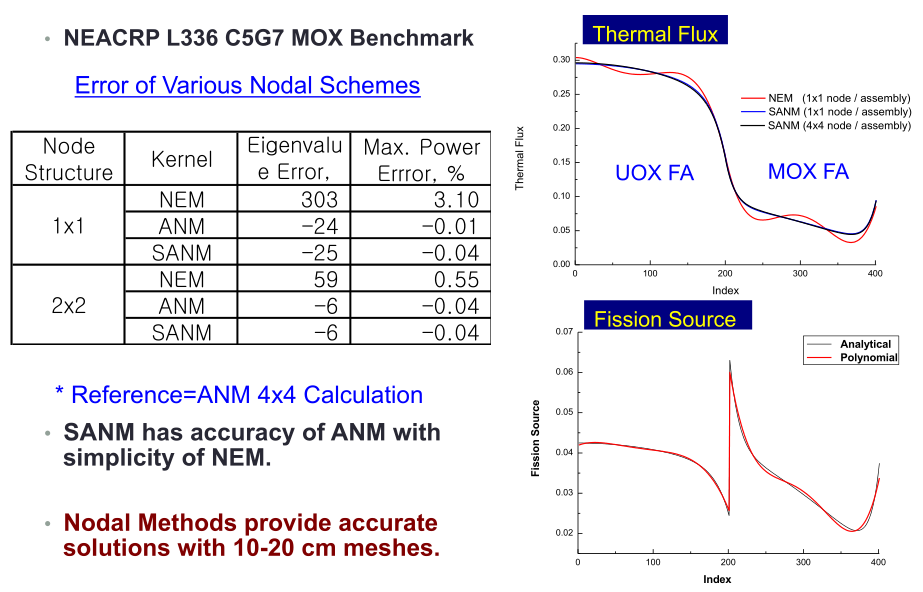
\includegraphics[width=5in]{images/methd/SANM-accuracy.png}
      \caption{Accuracy of SANM in Two-Group Application} \label{SANM-accuracy}
    \end{figure} 
  \end{enumerate}


\clearpage
\topic{Nonlinear Iterative Technique To Reduce Storage}
In this section we show how the three nodal methods come down to be pretty much the same. The classic solution sequance involves,
\begin{enumerate}
\item Guess $\keff$, approximate transverse leakages as zero.
\item Evaluate all coupling terms for 1-node equation,
  \eqn{ \left[ \begin{array}{c} J_1 \\ J_2 \end{array} \right] = \left[ \begin{array}{cc} a_{11} & a_{12} \\ a_{21} & a_{22} \end{array} \right] \left[ \begin{array}{c} \bar{\psi}_1^+ \\ \bar{\psi}_2^+ \end{array} \right]  - \left[ \begin{array}{cc} b_{11} & b_{12} \\ b_{21} & b_{22} \end{array} \right] \left[ \begin{array}{c} \bar{\psi}_1^- \\ \bar{\psi}_2^- \end{array} \right] + \Sum_{m=1,4} \left[ \begin{array}{cc} c_{11} & c_{12} \\ c_{21} & c_{22} \end{array} \right] \left[ \begin{array}{c} L_{m1} \\ L_{m2} \end{array} \right] }

\item Setup global matrix equation,
\eqn{ \left[ \begin{array}{cccc} 
 [A] & [B] & [C] & [D] \\
 \left[E\right] & [1] & [F] & [G] \\
 \left[H\right] & [I] & [1] & [J] \\
 \left[K\right] & [L] & [M] & [1] \\
\end{array} \right]  
\left[ \begin{array}{c} 
[\bar{\psi} ] \\ 
\left[L_x\right] \\ 
\left[L_y\right] \\ 
\left[L_z\right] \end{array} \right] = \frac{1}{\keff} 
\left[ \begin{array}{cccc} 
[m] & [0] & [0] & [0] \\ 
\left[0\right] & [0] & [0] & [0] \\ 
\left[0\right] & [0] & [0] & [0] \\ 
\left[0\right] & [0] & [0] & [0] 
\end{array} \right] 
\left[ \begin{array}{c} 
[\bar{\psi} ] \\ 
\left[L_x\right] \\ 
\left[L_y\right] \\ 
\left[L_z\right] \end{array} \right] }

\item We solve the 3D balance equation by fission source and flux/leakage iteration, similar to finite difference, but leakate term has group-to-group coupling. 
\item Update $\keff$ and return to 2 until converged. 
\end{enumerate}

Next \textbf{the non-linear iterative solution} sequence was developed,
\begin{enumerate}
\item  Guess $\keff$, solve the standard 3D finite difference equations. 

\item Evaluate all interface currents from 2-node equations,
  \eqn{ \left[ \begin{array}{c} J_1 \\ J_2 \end{array} \right] = \left[ \begin{array}{cc} a_{11} & a_{12} \\ a_{21} & a_{22} \end{array} \right] \left[ \begin{array}{c} \bar{\psi}_1^+ \\ \bar{\psi}_2^+ \end{array} \right]  - \left[ \begin{array}{cc} b_{11} & b_{12} \\ b_{21} & b_{22} \end{array} \right] \left[ \begin{array}{c} \bar{\psi}_1^- \\ \bar{\psi}_2^- \end{array} \right] + \Sum_{m=1,4} \left[ \begin{array}{cc} c_{11} & c_{12} \\ c_{21} & c_{22} \end{array} \right] \left[ \begin{array}{c} L_{m1} \\ L_{m2} \end{array} \right] }
It's almost finite difference, but higher order in the sense that we say if flux has already converged, what would the current be. 

\item Redefine equivalent coupling terms to preserve nodal solution for current. Notice the coefficients $\alpha, \beta, \gamma, \delta$ are non-linear functions of the solution. 
  \eqn{ \left[ \begin{array}{c} J_1 \\ J_2 \end{array} \right] = \left[ \begin{array}{cc} \alpha & 0 \\ 0 & \gamma \end{array} \right] \left[ \begin{array}{c} \bar{\psi}_1^+ \\ \bar{\psi}_2^+ \end{array} \right]  
- \left[ \begin{array}{cc} \beta & 0 \\ 0 & \delta \end{array} \right] \left[ \begin{array}{c} \bar{\psi}_1^- \\ \bar{\psi}_2^- \end{array} \right] }
This is almost CMFD. As we solve the problem, we will slowly find out the 4 coefficients and if the solution converges it should be identical to the original matrix problem. 


\item Set up global matrix equation,
  \eqn{ [A] [[\bar{\psi}]] = \frac{1}{\keff} [M] [[\bar{\psi}]] }

\item Solve 3D balance equations by fission source and flux iteration (same as finite-difference, and no group-to-group spatial coupling term). 

\item Update $\keff$ and return to 2 until converged. 
\end{enumerate}
This method is almost the same as CMFD, but with slightly different coefficients $\alpha, \beta, \gamma, \delta$. The point is, whether we do any one of the three nodal methods, we get a slightly different net current, the rest of the iteration looks the same. Mechanically, it is the same as the two-node two-group finite difference solution that we've already done. 




\clearpage
\topic{Solving the Eigenvalue Problem}

[FIXME]

Wielandt's fractional iteration: pro: faster; con: harder to invert the matrix. Though with the block formulism (and assume a large matrix), it is not any harder. 



\clearpage
\topic{Steady State Neutronics Algorithm}
How SIMULATE3 does steady state neutronics: [FIXME]
\begin{enumerate}
\item Non-linear iteration to get spatial coupling coefficients. 
\item 
\end{enumerate}

The overall steady-state iteration strategy. This would be covered in more details in 22.212. 

[FIXME] insert image. 

\clearpage
\topic{Summary of Transverse Integration Methods}
The major assumption we make is that quadratic transverse leakage is a good representation; it if not, we need to refine our mesh till quadratic expension is good for transverse leakage. 
\begin{enumerate}
\item Transverse integration method is an innovative way to solve 3D diffusion equation by converting 3D PDE into 3 ODEs: 
  \begin{itemize}
    \item Solutions are only weakly dependent on the leakage shapes;
    \item Transverse leakage is approximated by a second order polynomial and iteratively updated.
  \end{itemize}

\item NEM is simple and efficient; it facilitates multi-group calculations, but loses accuracy for highly varying flux problems. 

\item ANM has the best accuracy, but it is not easy (though has been done) for general multi-group problems.

\item SANM is the most practical for LWR applications, because it has simple algebra, is multi-group applicable, and is comparable in accuracy to ANM. 

\item Non-linear solution method (eg, iterative) can be easily applied to all three methods. 
\end{enumerate}



\clearpage

\end{document}
